\subsection{Beispiele Magnetisches Feld}
    \subsubsection{Leiterschleife mit verschiebbarem Bügel}
        ACHTUNG: Richtung der eingeführten Vektoren im Rechtssystem\\
        $\vec{l}$ in Richtung des Elektronenflusses
        \includegraphics[width = \linewidth]{src/images/leiterschleife_bügel_verschiebbar.png}
        \mathbox{d\vec{A} = d\vec{s} \times \vec{l} \rightarrow \frac{d \vec{A}}{dt} = \vec{v} \times \vec{l}}
        Induktionsgesetz:
        \begin{empheq}[box = \fbox]{align*}
            U_i &= -\frac{d}{dt} \int \vec{B} d\vec{A} = -\frac{d}{dt} \left( \vec{B} \vec{A} \right)\\
            &= \left(\vec{v} \times \vec{B} \right) \vec{l} - \vec{A} \frac{d \vec{B}}{dt}
        \end{empheq}
    
    \subsubsection{Beispiel Elektromotor}
        \begin{minipage}{0.54\linewidth}
            \begin{empheq}[box = \fbox]{align*}
                M &= I (\vec{A} \times \vec{B})\\
                M_{\text{dip}} &= \vec{m} \times \vec{B}\\
                W &= -\int M_{\text{dip}} d\alpha = \vec{m} \vec{B}
            \end{empheq}
            \begin{scriptsize}
                \begin{empheq}{align*}
                    \vec{A} &= \text{Vektor normal zu Fläche}\\
                    \vec{B} &= \text{mag. Flussdichte}\\
                    \vec{m} &= \text{mag. Dipolmoment}\\
                \end{empheq}
            \end{scriptsize}
        \end{minipage}
        \begin{minipage}{0.44\linewidth}
            "Kommutator" kehrt Polarisierung des Stroms nach halber Umdrehungen um, damit volle Umdrehung ermöglicht wird.
            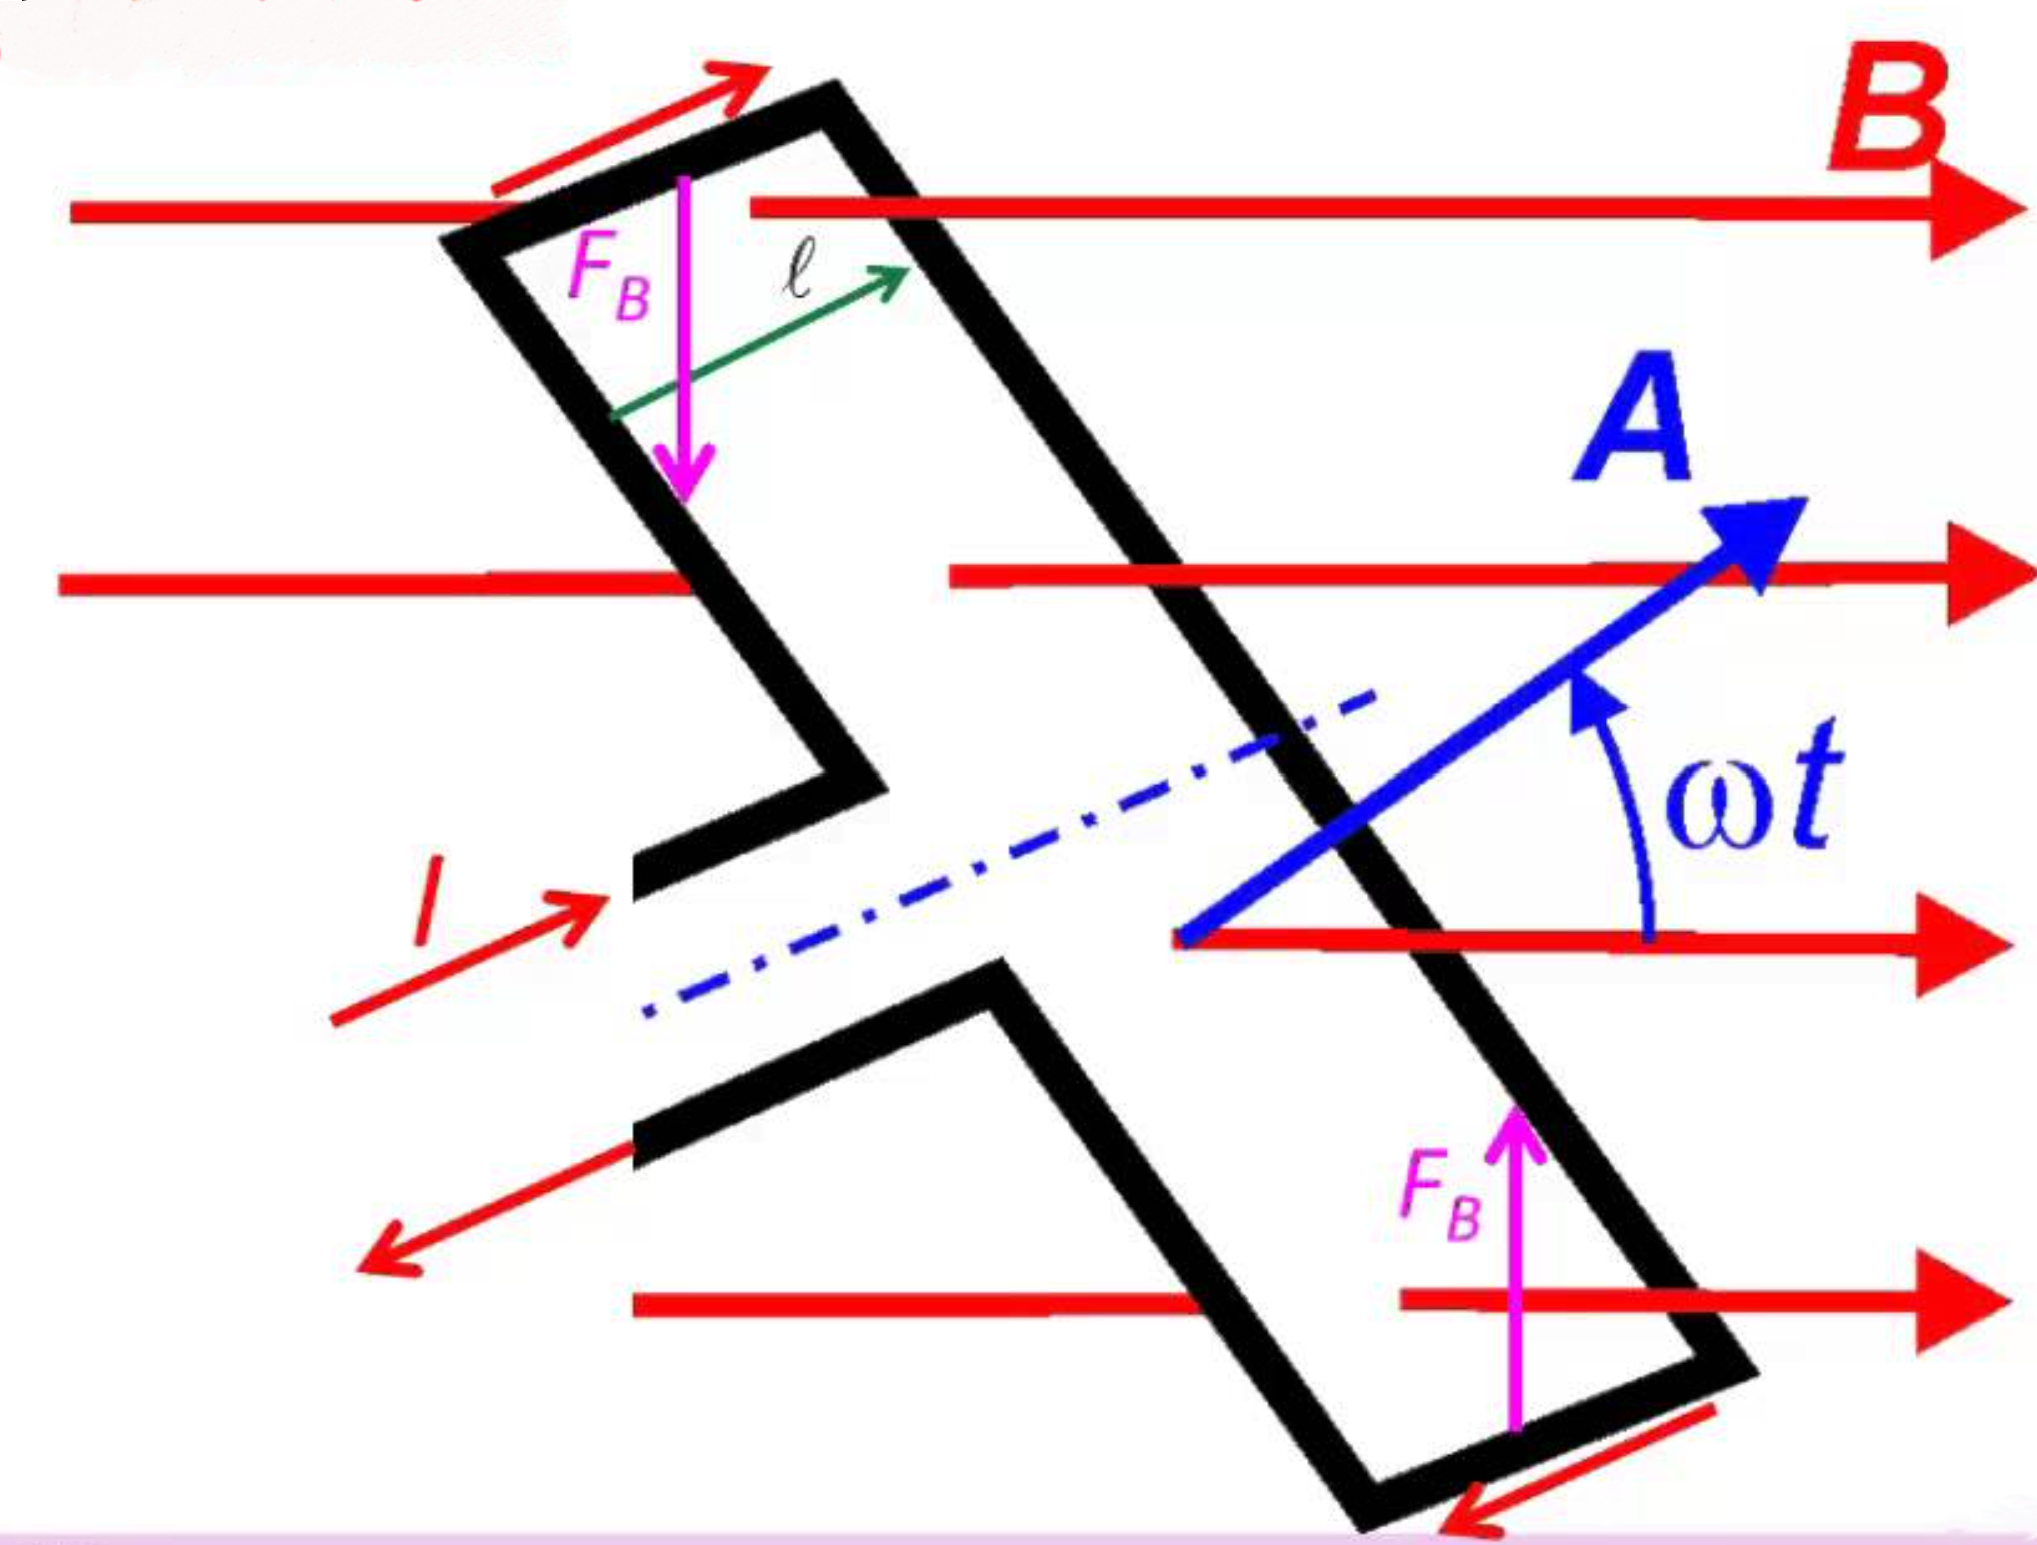
\includegraphics[width = \linewidth]{src/images/leiterschleife.png}
        \end{minipage}

    \subsubsection{Beispiel Transformator}
        \begin{minipage}{0.49\linewidth}
            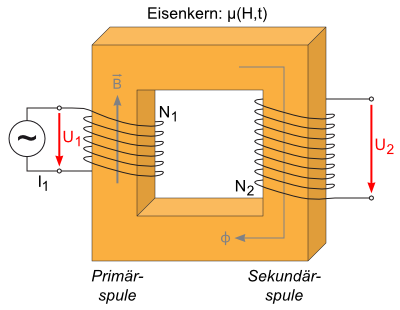
\includegraphics[width = \linewidth]{src/images/transformator.png}
        \end{minipage}
        \begin{minipage}{0.49\linewidth}
            \mathbox{\left| \frac{U_p}{U_s} \right| = \frac{n_p}{n_s}}
            \begin{scriptsize}
                \begin{align*}
                    p &= \text{Primärspule}\\
                    s &= \text{Sekundärspule}\\
                    U &= \text{el. Spannung}\\
                    n &= \text{Windungen}
                \end{align*}
            \end{scriptsize}
        \end{minipage}
%
    \subsubsection{Beispiel parallele stromdurchflossene Drähte}
        \begin{minipage}{0.49\linewidth}
            \includegraphics*[width = \linewidth]{src/images/magnetische_wirkung_draehte.png}
        \end{minipage}
        \begin{minipage}{0.49\linewidth}
            \begin{itemize}
                \item $\vec{I_1} \uparrow \uparrow \vec{I_2}$: anziehend
                \item $\vec{I_1} \uparrow \downarrow \vec{I_2}$: abstossend
            \end{itemize}
            \mathbox{F_1 = F_2 = \frac{\mu_0}{2 \pi} l \frac{I_1 I_2}{r}}
        \end{minipage}

    \subsubsection{Dynamo}
        Dynamo (Wechselspannung durch sich drehende Schleife in homogenem Magnetfeld):
        \mathbox{U_i = \omega B_0 A_0 sin(\omega t) = U_0 sin(\omega t)}